\RequirePackage{mmap}
\documentclass[12pt]{article}
\usepackage[utf8]{inputenc}
\usepackage{geometry}
\geometry{
  margin=1in,
}
\usepackage{amsmath,amsthm,amssymb, listings, color, bm}
\usepackage{mathtools}
\usepackage{changepage}% http://ctan.org/pkg/changepage
\usepackage{enumitem}
\usepackage{csquotes}
\usepackage{fancyhdr}
\usepackage[T1]{fontenc}
\usepackage{titlesec}
\usepackage[absolute]{textpos}
\usepackage[hidelinks]{hyperref}
\usepackage{fontspec}
\usepackage[linesnumbered,ruled]{algorithm2e}
\setmainfont{Latin Modern Roman}
%% \usepackage{setspace}
%% \doublespacing

\renewcommand{\P}{\mathbb{P}}
\newcommand{\E}{\bm{E}}
\newcommand{\Var}{\bm{Var}}
\newcommand{\ul}[1]{\underline{#1}}

\newtheorem{theorem}{Theorem}[section]
\newtheorem{corollary}{Corollary}[theorem]
\newtheorem{lemma}[theorem]{Lemma}
\theoremstyle{definition}
\newtheorem{definition}{Definition}[section]

\DeclareMathOperator*{\argmax}{arg\,max}
\DeclareMathOperator*{\argmin}{arg\,min}

\setlength{\parindent}{0.25in}

\newif\ifextra
\extrafalse

\title{}

\pagenumbering{arabic}

\begin{document}
\pagestyle{fancy}
\fancyhf{} % sets both header and footer to nothin
\cfoot{\thepage}
\renewcommand{\headrulewidth}{1pt}
\lhead{\fontsize{10}{12} \selectfont CSE 446: Machine Learning (Prof. Sham Kakade)\\\textbf{\emph{Section 4: Margin of Separation, SVD}} }
\rhead{\fontsize{10}{12} \selectfont Kaiyu Zheng (TA)\\ \today}

\section{Margin of Separation}
Here is how we derive the concept of \emph{margin}. Let's not make any assumptions at first. Suppose we have a group of data points $\{(x_i,y_i)\}_{i=1}^N$ where $x_i\in\mathbb{R}^L$ and $y_i=\{-1,+1\}$. For simplicity, let us focus on $\mathbb{R}^2$ as in Figure \ref{fig:margin_compute}.

\begin{figure}[h]
  \centering
  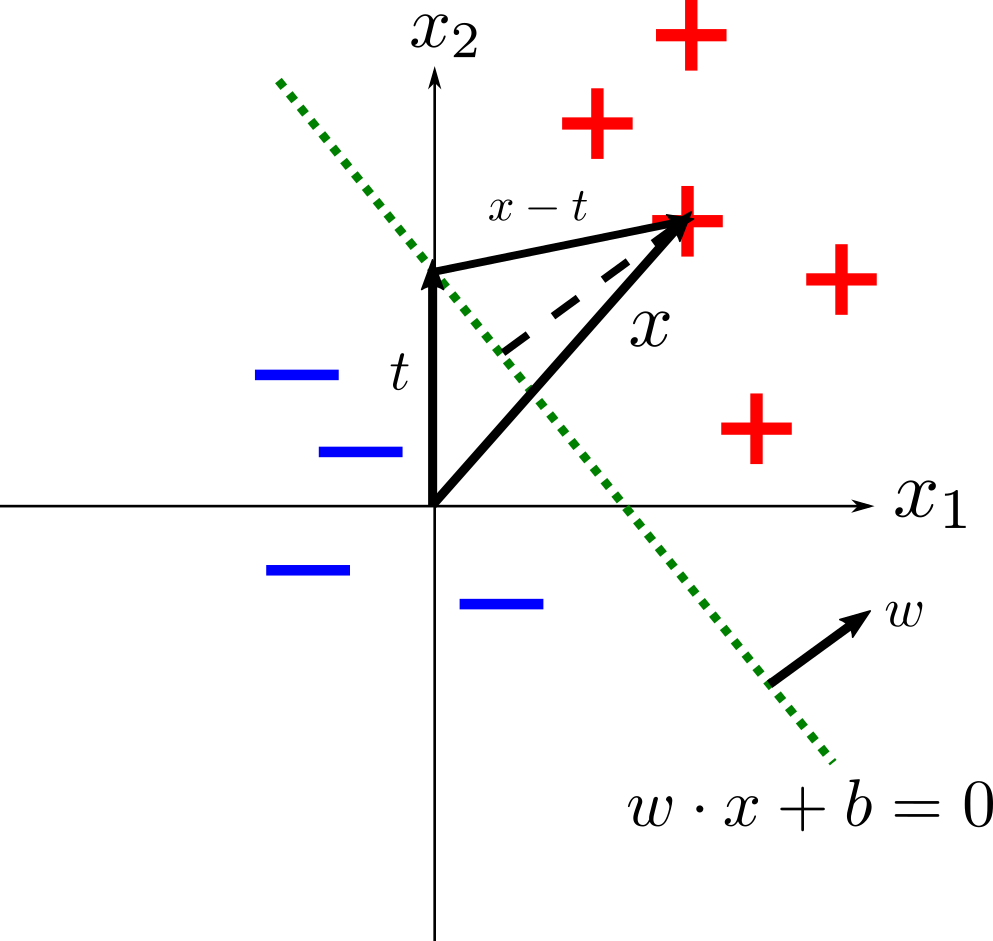
\includegraphics[scale=0.8]{figs/margin_compute}
  \caption{Deriving distance from data point to decision boudary.}
  \label{fig:margin_compute}
\end{figure}

As shown, we have positive and negative data points separated by a decision boundary (dashed line), given by $w\cdot x+b=0$, where $w\in\mathbb{R}^2$. The vector $x$ represents a data point, and $t$ is the vector from origin to the intercept with the $x_2$-axis.

It is straightforward that the distance from the data point to the decision boundary is
\begin{equation}
  d_{w,b}(x) = (x-t)\cdot\frac{w}{||w||}
\end{equation}
In the 2D case, we can write $w\cdot x+b=0$ as $w_1x_1+w_2x_2+b=0$. Therefore, the intercept at the $x_2$-axis is $-\frac{b}{w_2}$. So we have,
\begin{equation}
  t=[0,-\frac{b}{w_2}]^T
\end{equation}
In general (L-Dimensional space), the vector $t$ basically moves the decision boundary only along one axis, so $t= [0 , \cdots, 0 , -\frac{b}{w_i} , 0 , \cdots , 0]^T$. Therefore, we can simplify $d$ as follows
\begin{align}
  d_{w,b}(x) &= \frac{x\cdot w}{||w||}-\frac{t\cdot w}{||w||}\\
  &=\frac{x\cdot w}{||w||}-\frac{-\frac{b}{w_2}w_2}{||w||}\\
  &=\frac{w\cdot x}{||w||}+\frac{b}{||w||}
\end{align}
Now we have an equation for the (signed) distance between a data point to a decision boundary, which can be extended to beyond 2D.

Suppose the given decision boundary $l:w\cdot x+b=0$ separates the data $\mathcal{D}=\{(x_i,y_i)\}_{i=1}^N$. We care about how well the data is separated. That is, we care about the minimum distance between any point in $\mathcal{D}$ to $l$. If this distance is larger, then $l$ separates the data better. This distance can be written as:
\begin{equation}
\text{margin}(\mathcal{D},w,b)=\min_{\substack{w,b;\\(x_i,y_i)\in\mathcal{D}}}y_id_{w,b}(x_i)=\min_{\substack{w,b;\\(x_i,y_i)\in\mathcal{D}}}y_i\Big(\frac{w\cdot x_i}{||w||}+\frac{b}{||w||}\Big)
\end{equation}
We added $y_i$ to ensure the distance is positive. This value is defined as the \emph{margin} of separability. If the dataset cannot be linearly separated, then the margin is $-\infty$. The \emph{geometric margin} is defined as the largest margin the dataset can be separated with, denoted by $\gamma$
\begin{equation}
\gamma=\sup_{\substack{w,b}}\text{margin}(\mathcal{D},w,b)
\end{equation}
The CIML book does not have $||w||$ in the denominator of the margin. So its equation for geometric margin is wrong, since it needs the constrain $||w||=1$.

%define \emph{margin of separability}
%% \begin{align}
%% \text{margin(\mathcal{D},w,b)}=\left \{
%%   \begin{tabular}{ccc}
%%     \min_{w,b,x_i\in\mathcal{D}}d_{w,b}(x_i)
%%   3 & 3 & -8 
%%   \end{tabular}
%% \right \}
%% \end{align}
%% \end{definition}

%% \begin{figure}[h]
%%   \centering
%%   \includegraphics[scale=0.8]{figs/margin}
%%   \caption{Decision boundary and margin. Left: possible decision boundaries. Center: One possible decision boundary with margin $\gamma$. Right: decision boundary that best separates the data $\mathcal{D}$ (with largest margin $\gamma_{\mathcal{D}}$).}
%%   \label{fig:perceptron}
%% \end{figure}



\section{Singular Value Decomposition}

\textbf{\large Recap of eigenvectors, eigenvalues, and covariance matrix.}
\begin{definition}[Eigenvector and Eigenvalue]
Let $\bm{A}\in M_{n\times n}(\mathbb{R})$, then a nonzero vector $\bm{u}$ is an \emph{eigenvector} of $\bm{A}$ if there exists a scalar $\lambda$ such that $\bm{Au}=\lambda\bm{u}$. The scalar $\lambda$ is called the \emph{eigenvalue}
\end{definition}

$\bm{0}$ is never an eigenvector.

\begin{theorem}[Condition for an Eigenvalue]
Let  $\bm{A}\in M_{n\times n}(\mathbb{R})$. Then $\lambda$ is an eigenvalue of $\bm{A}$ if and only if $\bm{A}-\lambda\bm{I_n}$ is singular, i.e.
\begin{equation}
det(\bm{A}-\lambda\bm{I_n})=0.    
\end{equation}
We refer to $det(\bm{A}-\lambda\bm{I_n})=0$ as the \emph{characteristic polynomial}.
\end{theorem}

The intuition of eigenvectors is to think of them as the axis of the corresponding linear transformation. The eigenvalue $\lambda$ helps to know if $\bm{x}$ is stretched or shrunk, when multiplied by a matrix $\bm{A}$ (i.e. $\bm{Ax}$).

\paragraph{Covariance matrix} Suppose $X=[X_1,\cdots,X_n]$ is a vector of random variables. Then we define the covariance matrix $\Sigma$ of $X$ as (if $\mu_i=\E[X_i]$)
\begin{equation}
  \Sigma_{ij}=\text{cov}(X_i, X_j)=\E[(X_i-\mu_i)(X_j-\mu_j)]=\E[X_iX_j]-\mu_i\mu_j
\end{equation}

\noindent\underline{\textit{Facts about covariance matrix}}
\begin{itemize}
\item A covariance matrix $\Sigma$ is
  \begin{itemize}
  \item symmetric
  \item (therefore) diagonalizable
  \item (therefore) an $n\times n$ $\Sigma$ contains $n$ orthogonal eigenvectors.
  \end{itemize}
\end{itemize}

\noindent \textbf{Single Value Decomposition.}

\begin{theorem}
  For any given real matrix $A\in\mathbb{R}^{n\times m}$, there exists a unique set of matrices $U, S, V$ such that
  \begin{equation}
    A = USV^T
  \end{equation}
  where $U\in\mathbb{R}^{n\times n}$ and $S\in\mathbb{R}^{n\times p}$ and $V\in\mathbb{R}^{p\times p}$ $U^TU=I$ and $V^TV=I$. This is called the \emph{singular value decomposition} of $A$.
\end{theorem}
$U$ and $V$ are orthonormal matrices. $S$ is a diagonal matrix\footnote{More precisely, it is a rectangular diagonal matrix because $n$ may not equal to $p$. Still, $S_{ij}=0$ if $i\neq j$.}. The elements in $S$ are called \emph{singular values} of $A$. The eigenvectors of $A^TA$ are columns of $V$, and the eigenvectors of $AA^T$ are columns of $U$. The entries in $S$ are positive, and sorted in decreasing order ($S_{11}\geq S_{22}\geq\cdots$).\\

\noindent\textbf{Connection to principal component analysis.}

The goal of principal component analysis (PCA) is to represent observations $X\in\mathbb{R}^{n\times d}$ by $Z\in\mathbb{R}^{n\times k}$ such that $k<d$ and $Z$ \textbf{\emph{best preserves variance}} of $X$. In fact, the first $k$ principal components is the eigenvectors of the covariance matrix of the data with the $k$-highest eigenvalues. $\Sigma=UDU^T$, so the first $k$ columns of $U$ are the eigenvectors (orthonormal) with eigenvalues in the first $k$ entries of the diagonanl matrix $D$.

%% \bibliography{references}
%% \bibliographystyle{plain}

\end{document}

